\documentclass[10pt,a4paper,twocolumn]{article}
\usepackage[a4paper,left=2.25cm,right=2.25cm,top=2.0cm,bottom=2.1cm,columnsep=0.65cm]{geometry}
\usepackage[T1]{fontenc}
\usepackage[utf8]{inputenc}
\usepackage{newtxtext,newtxmath,microtype}
\renewcommand{\ttdefault}{cmtt}
\DeclareRobustCommand{\ttfamily}{\fontencoding{OT1}\fontfamily{cmtt}\selectfont}
\usepackage{graphicx,booktabs,amsmath,array,xcolor,url,natbib,tikz}
\usetikzlibrary{arrows.meta,positioning}
\usepackage[font=small,labelfont=bf]{caption}
\usepackage[breaklinks=true,hidelinks]{hyperref}
\definecolor{revision}{HTML}{B00020}
\definecolor{inkblue}{HTML}{185B83}
\newcommand{\rev}[2]{\par\smallskip\noindent\begin{minipage}{\linewidth}\color{revision}\footnotesize\textbf{REVISION #1.} #2\end{minipage}\par\smallskip}
\newcommand{\nd}{\texttt{non\_distinct}}
\newcommand{\wt}{\textsc{WorkTrace}}
\newcommand{\src}[1]{\path{#1}}
\setlength{\parindent}{1em}
\setlength{\parskip}{0pt}
\setlength{\textfloatsep}{10pt plus 2pt minus 2pt}
\setlength{\floatsep}{8pt plus 2pt minus 2pt}
\setlength{\intextsep}{9pt plus 2pt minus 2pt}
\renewcommand{\topfraction}{0.93}
\renewcommand{\bottomfraction}{0.85}
\renewcommand{\textfraction}{0.06}
\renewcommand{\floatpagefraction}{0.75}
\setcounter{topnumber}{3}
\setcounter{totalnumber}{5}
\setlength{\emergencystretch}{1em}
\title{\textbf{WorkTrace: How Coding Agents Explore,\\Change Code, and Check Their Work}}
\author{Anonymous working manuscript}
\date{Annotated research draft --- 26 October 2026}
\begin{document}
\maketitle
\begin{abstract}
Coding agents inspect files, change code, and run checks. Final success and tool-call counts do not show how agents organize this work. We present \wt, a four-stage framework for this analysis. It links each tool operation to a work target, an inferred code version, and earlier evidence. We study 6,300 runs from three models under one harness. We also study 6,000 runs from one model under three harnesses. The analysis shows two work patterns. First, Gemini performs more checks on the final code version than on earlier versions. This gap remains under three saved version rules. Second, OpenHands and SWE-agent revisit known targets more often than mini-swe-agent on the same tasks. Their mean revisit rates are 32.9\%, 30.0\%, and 18.2\%, respectively. Exact-repeat rates are close to 0.2\% for all three harnesses. These findings show where work accumulates and which system comparisons need closer inspection. They do not establish that the additional work is unnecessary. We explain how evidence about test scope and unresolved questions can support that next assessment.
\end{abstract}\par\medskip
\noindent\textit{Working-draft status.} This revision adds statistical analyses of saved data. It adds no agent runs or human labels. Red notes identify the next research steps.
\rev{01}{Repair the state-tracking errors before treating these results as final. The new analyses test saved measurements. They do not repair those measurements.}

\section{Introduction}
Coding agents often solve the same task through different sequences of work. One agent may inspect many files before an edit. Another may edit early and then run many checks. A final patch and a tool-call count cannot explain this difference.

We need to know where the work occurs. Does an agent check each code version, or mainly the final version? Does a harness return to known targets, even when it rarely repeats an exact command and output? These questions help researchers compare systems and choose cases for closer analysis.

TRACE provides a useful approach to such questions \citep{trace}. It first measures broad behavior, then reconstructs reasoning graphs, and then studies common patterns. It connects those patterns to intermediate answer correctness and further utility tests. Coding-agent traces require a different representation. Code changes during a run, and two different commands can test the same code property.

We introduce \wt\ to reconstruct this external work. The framework has four stages: collect operations, infer work relations, construct progression graphs, and compare graph patterns. Two linked views show target visits and code versions. Together, they connect exploration, code changes, and verification.

Our study has two comparison sets. The first compares three models on the same tasks under mini-swe-agent. The second compares three harnesses on the same tasks with Qwen fixed. The results support two findings:
\begin{itemize}
\setlength{\itemsep}{2pt}\setlength{\topsep}{3pt}
\item \textbf{Final-version checking.} Gemini places more checks on its final inferred code version than on an average earlier version. Luna and Terra show no similar positive gap.
\item \textbf{Target revisits.} OpenHands and SWE-agent return to known targets more often than mini-swe-agent. This difference remains when we use the same rate definition and match tasks.
\end{itemize}
The framework makes these patterns measurable. It also identifies the evidence needed to interpret them. More checks can improve coverage. A file revisit can answer a new question. We therefore separate an observed work pattern from a claim that the work is excessive.
\rev{02}{Keep these two findings central. Explain the decision each finding supports. Confirm the patterns on fresh tasks after the measurement repairs.}

\section{Related Work}
\paragraph{Work and reasoning structures.}
TRACE studies how proposed answers change during reasoning \citep{trace}. Bouzenia and Pradel study thought--action--result sequences in software agents \citep{bouzenia}. \wt\ studies targets, code versions, and evidence within the same run. These links support comparisons of where agents spend their work.
\paragraph{Redundant work and efficiency.}
RedundancyBench evaluates redundant steps and their supporting evidence \citep{redundancybench}. Its annotation procedures can inform our validation. AgentDiet reduces agent history \citep{agentdiet}. TRIM studies unnecessary changes in final patches \citep{trim}. These studies address related questions, but each uses a different outcome. A repeated observation, a removable history item, and an unnecessary code change are not interchangeable labels.
\paragraph{Interaction with users.}
SWE-TaskFlow studies how benchmark task delivery matches user task flows \citep{taskflow}. Such data can test how new requirements change an agent's work. Our current comparisons use fixed task instructions.
\rev{03}{Credit any annotation procedure adapted from RedundancyBench. Add an interaction study only if it tests an explanation of the two main findings.}

\section{Benchmark Agent Work}
We first compare final success and the amount of work. We then use \wt\ to locate that work within each run.
\subsection{Across Models}
The first set contains 700 tasks, three models, and three runs per task and model. All 6,300 runs use mini-swe-agent. The saved operation table contains 188,609 operations. We retain the model names in the source metadata: Gemini 3.7 Flash, GPT-5.6 Luna, and GPT-5.6 Terra.
\begin{table*}[t]
\centering\small\setlength{\tabcolsep}{8pt}
\begin{tabular}{lrrrrr}
\toprule
Model & Runs & Success (\%) & Calls/run & Input tokens (M) & Exact repeats (\%)\\
\midrule
Gemini 3.7 Flash & 2,100 & 60.0 & 53.1 & 3.34 & 2.21\\
GPT-5.6 Luna & 2,100 & 50.0 & 17.6 & 0.25 & 0.02\\
GPT-5.6 Terra & 2,100 & 54.2 & 19.0 & 0.24 & 0.05\\
\bottomrule
\end{tabular}
\caption{Saved cross-model benchmark on 700 matched tasks. Tokens and calls are per-run means. Exact repeats require the same normalized command and output. Their rates are means of per-run rates. Success means that the dataset marks the task as resolved.}
\label{tab:model}
\end{table*}
Gemini has higher final success and uses more calls than either GPT model (Table~\ref{tab:model}). This comparison does not show whether its additional work is useful. The models and their released settings differ. They also differ in the number of code versions and checks, which we study in Section~\ref{sec:findings}.

\subsection{Across Harnesses}
The second set uses Qwen3.8-27B from Open-SWE-Traces v1.2 \citep{openswe}. It contains 2,000 shared tasks with one selected run per harness. The three harnesses are mini-swe-agent, OpenHands, and SWE-agent. Together, the 6,000 runs contain 370,992 operations.
\begin{table*}[t]
\centering\small\setlength{\tabcolsep}{8pt}
\begin{tabular}{lrrrrr}
\toprule
Harness & Runs & Success (\%) & Calls/run & Exact repeats (\%) & Target revisits (\%)\\
\midrule
mini-swe-agent & 2,000 & 57.1 & 51.8 & 0.20 & 18.2\\
OpenHands & 2,000 & 51.0 & 66.2 & 0.18 & 32.9\\
SWE-agent & 2,000 & 54.5 & 67.5 & 0.20 & 30.0\\
\bottomrule
\end{tabular}
\caption{Cross-harness benchmark with Qwen fixed. This revision calculates all rates as means of per-run rates. Older saved summaries used pooled operation rates for revisits. The new values permit a consistent comparison.}
\label{tab:harness}
\end{table*}
OpenHands and SWE-agent use more calls than mini-swe-agent (Table~\ref{tab:harness}). All three have exact-repeat rates near 0.2\%. However, their target revisit rates differ. Section~\ref{sec:patterns} examines this difference with paired task comparisons.

\subsection{Reference-Patch Size}
We also compare work across reference-patch size quartiles (Figure~\ref{fig:patchsize}). Patch size is a proxy for task demands. It is not a direct measure of reasoning difficulty.
\begin{figure*}[t]
\centering\includegraphics[width=\textwidth]{images/patch_size_profiles.pdf}
\caption{Restored patch-size analysis. Q1 contains the smallest reference patches and Q4 the largest. The model set has 657 tasks with patch metadata: 165 in Q1 and 164 in each remaining bin. Each task has nine runs. The harness set has 500 matched tasks per bin and three runs per task. All rates are means of per-run rates. Lines show descriptive means without uncertainty intervals. Task sets differ between rows.}
\label{fig:patchsize}
\end{figure*}
Across the model set, pooled mean calls increase from 25.0 in Q1 to 34.4 in Q4. Mean success falls from 69.6\% to 37.5\%. Exact-repeat rates are 0.70\%, 0.75\%, 0.83\%, and 0.75\% across the four bins. These values do not support a steady increase in exact-repeat rates with patch size.

The harness profiles also separate more work from more exact repetition. All three harnesses use more calls on larger-patch tasks. Their revisit rates also rise between Q1 and Q4. These profiles motivate structural analysis, but do not establish excessive work. We keep the saved success-defined difficulty bins outside this comparison because their success trends follow from the bin definition.

\subsection{Comparison Method}\label{sec:comparison}
We analyze the model and harness sets separately because they contain different tasks. These sets cannot establish a model--harness interaction.

The additional analyses use 5,000 task-bootstrap samples with seed 20261026. Each sample draws tasks with replacement and keeps their associated runs together. Paired comparisons keep the same task on both sides. We report 95\% percentile intervals. These are exploratory intervals, without adjustment for multiple comparisons.

For the version analysis, we require at least two inferred versions and a final version other than the initial repository state. We then select task--repeat pairs that meet this rule for every model under every version rule. This gives 892 matched pairs from 418 tasks, with 892 runs per model. This selected subset tests whether the pattern persists under common conditions. It does not represent every run.
\rev{04}{Report all exclusions and settings in the final release. The saved metadata includes 4,198 missing results. Identify their causes before claiming complete observations.}

\section{Framework for Work Progression}
\wt\ maps a tool sequence into a description of the work. Table~\ref{tab:terms} defines the main terms.
\begin{table}[t]
\centering\small
\begin{tabular}{p{.21\columnwidth}p{.67\columnwidth}}
\toprule
Term & Meaning in this paper\\
\midrule
Operation & One native tool call and its recorded result.\\
Target & The file, command, or tool object that an operation addresses.\\
Revisit & An operation with an earlier same-target candidate.\\
Version & An inferred code state after a detected change.\\
Check & A run operation attached to a version, excluding detected read-only inspections.\\
Non-distinct & The annotator finds no new contribution relative to the cited earlier evidence.\\
\bottomrule
\end{tabular}
\caption{Terms describe recorded work. A check is not automatically a test, and a revisit is not automatically redundant.}
\label{tab:terms}
\end{table}
\begin{figure*}[t]
\centering
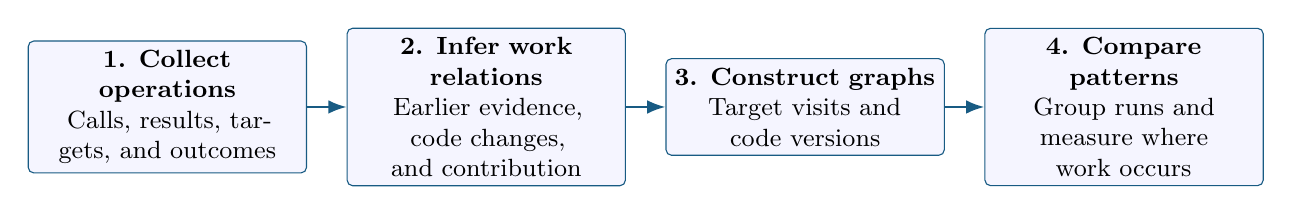
\begin{tikzpicture}[>=Latex,stage/.style={draw=inkblue,rounded corners=2pt,fill=blue!4,text width=3.3cm,align=center,minimum height=1.2cm,font=\small}]
\node[stage] (a) at (0,0) {\textbf{1. Collect operations}\\Calls, results, targets, and outcomes};
\node[stage] (b) at (4.05,0) {\textbf{2. Infer work relations}\\Earlier evidence, code changes, and contribution};
\node[stage] (c) at (8.1,0) {\textbf{3. Construct graphs}\\Target visits and code versions};
\node[stage] (d) at (12.15,0) {\textbf{4. Compare patterns}\\Group runs and measure where work occurs};
\draw[->,thick,inkblue] (a)--(b);\draw[->,thick,inkblue] (b)--(c);\draw[->,thick,inkblue] (c)--(d);
\end{tikzpicture}
\caption{Four stages of \wt. Operation IDs connect both graph views to the source records. The graphs summarize external actions. They do not reveal hidden model reasoning.}
\label{fig:pipeline}
\end{figure*}

\subsection{Stage 1: Collect Operations}
We use saved tool traces from the two comparison sets. The parser records each call, its result, its position, and the available exit status. It assigns operation types such as read, search, edit, run, and submit.

The parser also splits shell chains to inspect their parts. The native call remains the measurement unit. A call can contain several action types. Normalization removes selected volatile fields from execution outputs. Exact-repeat detection compares the normalized command and output hash.

\subsection{Stage 2: Infer Work Relations}
For each operation, the framework retrieves two possible earlier matches. One is the latest operation on the same target. The other is the latest same-type operation with the same usable output. The current rules exclude short or explicitly truncated outputs from the second search.

Rule facts describe whether the output matches and whether code may have changed. An automatic annotator then labels the operation's role, relation, and contribution. Roles include exploration, revision, and verification. Relations include unmatched, revisit, reproduction, and uncertain. Contributions can be distinct, non-distinct, or uncertain.

The validator requires a cited match for a non-distinct label. Thus, the labels measure contribution within the retrieved evidence. They do not measure all unnecessary work. Appendix~\ref{app:validation} reports the current annotation checks.
\rev{05}{Test candidate recall with independent readers who can inspect any earlier operation. The current rules prevent unmatched operations from receiving a non-distinct label.}

\subsection{Stage 3: Construct Progression Graphs}
\paragraph{Target graph.}
Each node represents a work target. Directed edges follow the operation sequence. Consecutive visits to one target form a self-loop. A later return forms a return edge. These edges locate repeated attention without assuming repeated information.

For example, an agent can read two different ranges of one file. The target repeats, but the second range can supply new evidence. Target identity also depends on the tool interface. A structured editor may expose a file path directly. A shell command may encode that path within a more specific expression.

\paragraph{Version graph.}
Each node represents an inferred code version. Detected code changes create new versions. Checks attach as self-loops to the version on which they run. Recognized restores can return to earlier versions.

A new node after a failed check receives the stored rule label \texttt{correct}. This label means revision after failure. It does not mean the resulting code is correct. Only final task success has a dataset outcome.

We retain three saved version rules. The first creates a version for every detected write, including uncertain writes. The second uses known writes only. The third excludes writes confined to inferred support files. Support files include temporary diagnostic scripts. The third rule uses final submission metadata, so it is a retrospective analysis.
\rev{06}{Fix false state matches, branch changes, unknown side effects, failed restores, and incomplete diffs. Rebuild the graphs before making final claims about version counts or backtracks.}

\subsection{Stage 4: Compare Patterns}
We group version graphs by model and version count. New versions advance horizontally. A new path after a backtrack moves to a higher row. Graphs align by these coordinates.

Node and edge weights record how often each component appears. The saved figures retain components present in at least 30\% of grouped runs. We display groups with at least 20 runs. This procedure follows TRACE's coordinate-based aggregation approach \citep{trace}.

We also calculate measures before graph pruning. The verification gap compares final-version checks with the mean checks on earlier versions. The revisit rate divides operations with a same-target candidate by all operations in a run. These measures support direct comparisons beyond visual inspection.
\rev{07}{Test the graph alignment and pruning thresholds. A simple-looking aggregate can hide uncommon paths. Use unpruned run measures for numerical findings.}

\section{Findings}\label{sec:findings}
\subsection{Work Progression Patterns}\label{sec:patterns}
TRACE's Explorer and Late Landing patterns depend on intermediate answer correctness \citep{trace}. Our data lacks intermediate code-correctness labels. We therefore name our patterns by the work that we observe.

\paragraph{Pattern I: Final-version checking.}
Gemini performs more checks on its final inferred version than on an average earlier version. Figure~\ref{fig:patterns} shows this pattern in the saved four-version groups. We test it numerically on the common subset defined in Section~\ref{sec:comparison}.
\begin{figure}[t]
\centering\includegraphics[width=\columnwidth]{images/patterns_four_versions.pdf}
\caption{Saved four-version patterns. R is the initial repository state. Blue loops show mean checks at each coordinate. Percentages show node presence. Dashed circles mark frequently final nodes. Rare components are pruned. These graphs do not mark correctness.}
\label{fig:patterns}
\end{figure}
For run $r$, we define the verification gap as
\begin{equation}
G_r=C_{r,\mathrm{final}}-\frac{1}{|V_r^-|}\sum_{v\in V_r^-}C_{r,v},
\end{equation}
where $C_{r,v}$ counts checks on version $v$. The set $V_r^-$ contains other inferred versions and excludes the initial repository state. A positive gap means more checks on the final version.

Under the support-file exclusion rule, Gemini averages 3.15 final checks and 0.61 checks per earlier version. Luna averages 0.39 and 0.43. Terra averages 0.47 and 0.57. These values use the same 892 task--repeat pairs per model.

Gemini's mean gap exceeds Luna's by 2.58 checks [2.30, 2.84]. It exceeds Terra's by 2.64 checks [2.37, 2.92]. The direction remains under the other two version rules (Figure~\ref{fig:comparisons}a). The Gemini--Luna contrast ranges from 1.80 to 2.58 checks across these rules.
\begin{figure*}[t]
\centering\includegraphics[width=.99\textwidth]{images/matched_comparisons.pdf}
\caption{New analyses of saved data. (a) Verification gaps under three version rules on a fixed subset of 418 tasks. Each model has 892 runs. (b) Mean revisit rates on the same 2,000 tasks for each harness. Bars and points use 95\% task-bootstrap intervals. Both plots describe the current measurements, before state-tracking repairs.}
\label{fig:comparisons}
\end{figure*}
The gap also appears in both resolved and unresolved Gemini runs. Under support-file exclusion, their mean gaps are 2.46 [2.19, 2.73] and 2.48 [2.12, 2.85], respectively. These groups use all eligible Gemini runs, rather than the common subset. The association therefore does not require final task success.

\textbf{What this explains.} Gemini's additional execution work includes a final-version checking phase. Total call counts cannot locate that phase. The graph can. However, the final version can fail the task. Its position does not establish correctness or sufficient verification.
\rev{08}{Identify which properties each check tests. Compare new coverage, repeated coverage, and stochastic reruns. Measure the time available for checks before interpreting the gap as excessive verification.}

\paragraph{Pattern II: Target revisits.}
With Qwen fixed, the harnesses differ in how often they return to known targets. Mean revisit rates are 18.2\% for mini-swe-agent, 32.9\% for OpenHands, and 30.0\% for SWE-agent. These use one consistent per-run definition (Figure~\ref{fig:comparisons}b).

Paired comparisons give an OpenHands--mini-swe-agent gap of 14.73 percentage points [14.26, 15.19]. The SWE-agent--mini-swe-agent gap is 11.81 points [11.37, 12.25]. Removing the task with 164 repeated probe executions changes these gaps to 14.76 and 11.85 points. The direction also holds within both source datasets (Appendix~\ref{app:additional}).

Exact-repeat contrasts are much smaller. Relative to mini-swe-agent, the mean differences are $-0.013$ points for OpenHands and $+0.004$ points for SWE-agent. Their intervals include zero. This does not establish equivalence, but it shows that exact repeats alone miss the much larger revisit contrast.

\textbf{What this explains.} The harnesses organize recorded target access differently. They can revisit a file through a new command or a new range. Tool interfaces also change how the parser identifies targets. Thus, the pattern identifies a comparison that requires evidence inspection. It does not prove memory failure or excessive exploration.
\rev{09}{Normalize file paths, read ranges, and mixed calls across harnesses. Then inspect whether the remaining revisits resolve new questions or return to questions already settled.}

\subsection{Trace the Evidence}
A graph shows where to inspect. Evidence about an operation shows what we can conclude from it.
\paragraph{Do later final-version checks use new commands?}
The saved Gemini reconciliation contains 6,699 final-version checks across 2,100 runs. A run's first check is automatically a new command within that version. We remove this first check from each nonempty run before assessing later checks.

The remaining 4,964 checks include 89.0\% new commands [87.5, 90.5]. Identical command-and-output reruns account for 2.6\% [2.1, 3.1]. Same-command checks with different outputs account for 8.4\% [7.1, 9.8]. These rates pool checks and resample tasks.

Thus, most later checks are not exact reruns. But command variety does not establish new test coverage. Two pytest commands can select overlapping tests. Different tests can exercise the same property. This evidence supports a checking phase, while leaving its benefit unresolved.
\rev{10}{Extract test IDs, assertions, configuration, and relevant code changes. Replace command variety with a measure of the evidence each check adds.}

\paragraph{Do revisits add new information?}
The 50-run model pilot contains 1,432 operations. Of 225 operations with retrieved candidates, 51 receive a non-distinct label. Only 21 receive both reproduction and non-distinct labels. Those 21 are candidates for redundancy under the current evidence rules.

The 60-run Qwen pilot contains 4,018 operations. Non-distinct shares among operations with candidates are 5.1\% for mini-swe-agent, 5.2\% for OpenHands, and 9.7\% for SWE-agent. These small pilot estimates cannot establish the meaning of every revisit in the 6,000-run set.

The important next distinction is whether a revisit addresses an unresolved question. A return can confirm a code change, inspect another file range, or recover missing context. Each case requires the operation and its earlier evidence. Graph shape alone cannot decide which case applies.
\rev{11}{Build an independent human reference for matched and unmatched operations. Include new ranges, relevant code changes, missing outputs, and valid matches outside the retrieved candidates.}

\subsection{Towards Managing Excess Work}
We use \emph{excessive work} to mean continued work whose expected benefit is too small for its cost, under a stated decision rule. This definition requires an outcome and a cost. Counts and loops provide candidates for assessment.

\paragraph{What the current framework identifies.}
The current graphs locate repeated checking and repeated attention. Evidence-linked labels can mark operations with no new contribution relative to a retrieved match. These are candidate signals. They do not cover all forms of excessive work.

For example, an agent can inspect many new files after it already has sufficient evidence to act. Each read can reveal new facts while adding little value to the task. A novelty label alone will miss this form of excessive exploration.

\paragraph{Proposed assessment layer.}
The next layer must attach operations to explicit work units. For exploration, a work unit is a question or hypothesis supported by the visible trace. For verification, it is a code property to check. We must retain uncertainty when the trace does not identify that unit.

For each operation, record four items: the work unit, the relevant state, the available earlier evidence, and the remaining uncertainty. Then assess whether the result changes a task-relevant decision. Current purpose strings and contribution labels do not reliably supply all four items. This layer is a proposed extension, not a completed annotation result.

\paragraph{Verification assessment.}
Flag a candidate when a check addresses the same property on an unchanged relevant state. Inspect whether it adds coverage or justified confidence. The state includes code, test selection, configuration, and external conditions.

For example, running the same deterministic test with different output flags can repeat the same evidence. Running a previously untested edge case can add evidence on the same code version. An identical stochastic rerun can also improve confidence. A verification loop becomes evidence of excess only after this benefit assessment under the stated criterion.

\paragraph{Exploration assessment.}
Flag a candidate when an operation revisits a settled question or pursues a new question with no justified role in the task. Check the information and plausible alternatives available before the operation. Eliminating a plausible cause is useful even if the inspected file is absent from the final patch.

For example, different searches can repeatedly locate a definition already found and inspected. These commands can belong to one settled work unit. By contrast, a new search can test another plausible caller and resolve an open question. The target graph locates the sequence. The work-unit and evidence records support the judgment.

\paragraph{Evidence required for the claim.}
We distinguish three levels. A graph pattern locates a candidate. Independent review can support a judgment of low benefit under a defined criterion. A controlled continuation experiment can test whether avoiding the work preserves success and reduces cost. These levels answer different questions.

\paragraph{Use of the framework.}
The version view locates checking phases. The target view locates repeated attention. Evidence links then distinguish new information from repeated information. This sequence gives a clear use for the framework: choose comparable cases, inspect the reason for the difference, and test the proposed explanation.
\rev{12}{Add the work-unit assessment layer and validate its judgments. Then compare diagnoses with simple summaries and with WorkTrace. Include novel but task-irrelevant exploration.}

\paragraph{Next experiment.}
A controlled continuation experiment can test whether a warning identifies removable work. At a selected prefix, compare continued work with a suitable alternative. Measure final success and total cost, including analysis overhead. Removing recorded operations while keeping the recorded suffix fixed is not an adaptive agent experiment.
\rev{13}{No stopping or work-removal result is available. Set the success and cost criteria before the experiment. A nonsignificant success difference does not prove preserved performance.}

\section{Conclusion}
\wt\ reconstructs how coding agents inspect targets, change code, and check versions. The current data shows two patterns: Gemini concentrates more checks on the final inferred version, and the Qwen harnesses differ in target revisits. New paired analyses preserve these differences under the tested measurement choices.

These patterns make system comparisons more specific. They identify where work accumulates and which evidence needs inspection. Independent validation and corrected state tracking remain necessary before using the framework to measure excessive work.
\rev{14}{After validation, rewrite the main claim around what the framework explains. Keep the two findings and their evidence clear. Do not transfer TRACE's correctness-based conclusions without an intermediate correctness measure.}

\section*{Limitations}
\paragraph{Measurement.}
The audit reproduces errors in state identity, branch changes, mutation targets, restore outcomes, and incomplete diffs. These errors can change the version graphs. The new sensitivity analyses use existing measurements and cannot establish that the errors are harmless.
\paragraph{Validation.}
Automatic annotators agree on many labels, but the intended human reference remains incomplete. Candidate retrieval restricts the labels. The external CodeTraceBench result is unfavorable and appears in Appendix~\ref{app:validation}.
\paragraph{Scope.}
Version matching selects runs with particular observed behavior. Target identifiers depend on tool interfaces. The two comparison sets use different tasks and released configurations. We therefore report system associations rather than isolated model or harness causes.
\paragraph{Utility.}
We do not observe intermediate patch correctness or the outcomes of stopping early. We also lack a complete monetary or time cost for every operation. Additional checks and revisits must not be counted as wasted work by default.

\begin{thebibliography}{9}
\small
\bibitem[Zhang et~al.(2026)]{trace}
Xinliang Frederick Zhang, Anhad Mohananey, Alexandra Chronopoulou, Pinelopi Papalampidi, Somit Gupta, Tsendsuren Munkhdalai, Lu Wang, and Shyam Upadhyay. 2026.
\newblock Do LLMs Really Need 10+ Thoughts for ``Find the Time 1000 Days Later''? Towards Structural Understanding of LLM Overthinking.
\newblock In \emph{Proceedings of ACL}, pages 17005--17030. \url{https://aclanthology.org/2026.acl-long.773/}.
\bibitem[Bouzenia and Pradel(2025)]{bouzenia}
Islem Bouzenia and Michael Pradel. 2025.
\newblock Understanding Software Engineering Agents: A Study of Thought-Action-Result Trajectories.
\newblock \url{https://www.software-lab.org/publications/ase2025_trajectories.pdf}.
\bibitem[Zhu et~al.(2026)]{redundancybench}
Liang Zhu, Bo Yang, Zhinuo Zhou, Jiachen Liang, Jiahao Guo, Yiyang Yin, Xiongwei Han, and Minyang Hu. 2026.
\newblock Redundant or Necessary? A Benchmark for Detecting Redundant Steps in Agent Trajectories.
\newblock arXiv:2605.29893v2. \url{https://arxiv.org/abs/2605.29893v2}.
\bibitem[Xiao et~al.(2026)]{agentdiet}
Yuan-An Xiao, Pengfei Gao, Chao Peng, and Yingfei Xiong. 2026.
\newblock Reducing Cost of LLM Agents with Trajectory Reduction.
\newblock arXiv:2509.23586v2. \url{https://arxiv.org/abs/2509.23586v2}.
\bibitem[Mathai et~al.(2026)]{trim}
Alex Mathai, Shobini Iyer, Aleksandr Nogikh, Petros Maniatis, Franjo Ivan\v{c}i\'{c}, Junfeng Yang, and Baishakhi Ray. 2026.
\newblock TRIM: Reducing AI-Generated CodeSlop via Agent Trajectory Minimization.
\newblock arXiv:2607.18161. \url{https://arxiv.org/abs/2607.18161}.
\bibitem[Slinko et~al.(2026)]{taskflow}
Igor Slinko, Yaroslav Golubev, and Sergey Titov. 2026.
\newblock Opinion: Coding-Agent Benchmarks Should Match Their Users' Task Flows.
\newblock arXiv:2610.09633v2. \url{https://arxiv.org/abs/2610.09633v2}.
\bibitem[NVIDIA(n.d.)]{openswe}
NVIDIA. n.d. Open-SWE-Traces, v1.2 dataset release.
\newblock \url{https://huggingface.co/datasets/nvidia/Open-SWE-Traces}.
\bibitem[NJU-LINK(n.d.)]{codetracebench}
NJU-LINK. n.d. CodeTraceBench, dataset release.
\newblock \url{https://huggingface.co/datasets/NJU-LINK/CodeTraceBench}.
\end{thebibliography}

\appendix
\section{Validation}\label{app:validation}
\paragraph{Automatic annotation.}
The primary annotator is recorded as DeepSeek-V4.1-Flash through the configured endpoint. The JetBrains pilot has 50 runs from 17 tasks. The Qwen pilot has 60 runs from 20 tasks. Larger partial label files are excluded from these pilot results.

A secondary annotator, GLM-5.3-Flash, labels 225 matched items and 200 sampled unmatched items from the JetBrains pilot. Matched contribution agreement is 90.2\%, with $\kappa=0.70$. Matched relation agreement is 84.0\%, with $\kappa=0.50$. Candidate-redundancy agreement across 425 items has $\kappa=0.83$. Three primary-model samples give contribution $\kappa=0.88$--0.90 on matched items.

These checks measure agreement. They do not establish accuracy. Both annotators receive the same candidates and rule facts. The 200-item human packet has no adjudicated contribution labels.
\paragraph{External comparison.}
The saved CodeTraceBench analysis includes 484 trajectories, 17,317 steps, and 69 human-labeled unuseful steps \citep{codetracebench}. Table~\ref{tab:ctb} reports the result. Only 32 of the 69 human-labeled steps have a retrieved WorkTrace candidate.
\begin{table}[htbp]
\centering\small
\begin{tabular}{lrrr}
\toprule
Predictor & Predicted & Precision & Recall\\
\midrule
Exact repeat & 412 & 5.6\% & 33.3\%\\
Target revisit & 4,599 & 0.6\% & 39.1\%\\
Candidate redundant & 536 & 3.5\% & 27.5\%\\
\bottomrule
\end{tabular}
\caption{Saved comparison against unuseful-step labels. These labels differ from WorkTrace's contribution construct. The result still provides no positive external validation.}
\label{tab:ctb}
\end{table}
\paragraph{Return after a detour.}
The saved pilot includes 153 returns after visits to other targets. Removing two uncertain contributions leaves 151 returns, 32 non-distinct labels, and 17 task clusters. A task-clustered GEE gives adjusted odds ratios of 32.7 [2.3, 456] for two to three intervening targets. The estimate for four or more is 14.5 [1.1, 193], relative to one target. The model controls run position, run length, and model identity. The intervals are wide, and the pattern mainly occurs in long runs. We retain this as a secondary exploratory result.
\begin{figure}[t]
\centering\includegraphics[width=\columnwidth]{images/return_profiles.pdf}
\caption{Restored return analysis using saved v2 labels. A detour counts distinct intervening targets. Points show non-distinct shares and saved task-bootstrap intervals. Bins contain 3--76 operations. One Luna interval cannot be estimated from the saved sample. The small, uneven groups do not establish a monotonic effect or excessive exploration.}
\label{fig:returns}
\end{figure}

\section{Additional Analyses}\label{app:additional}
\paragraph{Version sensitivity.}
Table~\ref{tab:sensitivity} uses the same 892 task--repeat pairs under all three rules. Every model has 892 runs from 418 tasks. Each contrast subtracts Luna's within-run verification gap from Gemini's gap.
\begin{table}[htbp]
\centering\small
\begin{tabular}{lrr}
\toprule
Version rule & Difference & 95\% interval\\
\midrule
All writes & 1.80 & [1.54, 2.05]\\
Known writes only & 2.21 & [1.94, 2.48]\\
Exclude support files & 2.58 & [2.30, 2.84]\\
\bottomrule
\end{tabular}
\caption{Paired Gemini--Luna contrasts in checks. Sensitivity to version rules changes the size but not the direction. All rules share unresolved implementation risks.}
\label{tab:sensitivity}
\end{table}
\paragraph{Source-dataset sensitivity.}
The matched harness set contains 1,063 Scale-SWE tasks and 937 SWE-rebench-V2 tasks. Table~\ref{tab:source} compares each harness with mini-swe-agent within a source dataset.
\begin{table}[htbp]
\centering\small\setlength{\tabcolsep}{3pt}
\begin{tabular}{llrl}
\toprule
Source & Harness & Gap & 95\% interval\\
\midrule
Scale-SWE & OpenHands & 16.60 & [15.96, 17.23]\\
Scale-SWE & SWE-agent & 11.80 & [11.17, 12.39]\\
SWE-rebench & OpenHands & 12.60 & [11.93, 13.27]\\
SWE-rebench & SWE-agent & 11.82 & [11.21, 12.45]\\
\bottomrule
\end{tabular}
\caption{Paired differences in mean revisit rates, in percentage points. The direction holds within both sources under the current target definition.}
\label{tab:source}
\end{table}
\paragraph{Exploration and uncertainty.}
These are additional analyses of data already used to develop the framework. Their intervals describe sampling variation under the stored measurements. They do not include parser error, annotator error, or the effect of selecting findings after inspection. Fresh tasks are required for confirmation.

\section{Data and Reproduction}
\paragraph{Saved inputs.}
The model benchmark uses \src{results/v2/benchmark/table1_by_model.csv}. The new harness analysis uses \src{results/v2/task5/runs_benchmark.parquet}. Version analyses use the three saved \src{runs_all.csv} files under \src{results/v2/viewb/}. The final-check analysis uses \src{results/v2/reconcile/scale_per_run.csv}.

Pilot results use \src{results/v2/task2/}, \src{results/v2/task3/}, \src{results/v2/task4/}, and \src{results/v2/qwen/pilot/}. The figure script redraws the saved four-version aggregates. It does not infer new graphs.
\paragraph{New outputs.}
The script \src{paper/worktrace-draft/analyze_saved_data.py} writes to \src{results/paper_revision_20261026/}. It produces paired contrasts, version sensitivity tables, outcome strata, source strata, and final-check categories. Assertions check sample sizes, matching, and count identities. The output manifest records the seed, package versions, and input hashes.
\paragraph{Dataset versions.}
JetBrains records revision \texttt{a5ec6ad84287}. Open-SWE records \texttt{a85dc97891bd}. The manuscript manifest retains the full hashes. Raw traces and some earlier caches are absent from this checkout.
\rev{15}{Release the full input-to-output map with parser, prompt, and dataset versions. Preserve complete observations so others can inspect the evidence behind each label.}

\section{One-Week Revision Priorities}
\paragraph{Days 1--2: Repair measurements.}
Fix the seven reproduced audit cases. Rebuild state facts and version graphs. Report how the fixes change both main findings.
\paragraph{Days 3--4: Validate evidence.}
Prepare an independent reference across models and harnesses. Include unmatched operations and difficult cross-tool cases. Keep uncertainty when the trace cannot support a judgment.
\paragraph{Days 5--6: Test explanations.}
Measure test scope for final-version checks. Normalize target access across harnesses. Compare simple summaries with the full framework on independently judged cases.
\paragraph{Day 7: Consolidate the study.}
Update the figures and main claims. Define a fresh-task confirmation set. Add a continuation experiment only if the required environment and budget are available.
\rev{16}{Prioritize reliable measurements and a direct test of the framework's value. More labels or a larger graph gallery alone will not resolve the main weaknesses.}
\end{document}
